\begin{center}

\includegraphics[width=0.6\textwidth]{content/3/chapter5/images/29.png}\\
Cippi在做杯子
\end{center}

\begin{tcolorbox}[breakable,enhanced jigsaw,colback=blue!5!white,colframe=blue!75!black,title={缺少编译器支持}]
	
截止到2020年底,没有C++编译器支持格式化库。感谢Victor Zverovich的原型库\href{https://github.com/fmtlib/fmt}{fmt},我可以用它进行实验。该库托管在\href{https://godbolt.org/z/Eq5763}{Compiler Explorer}上。当三大编译器GCC、Clang或MSVC中的一个支持C++20格式库,我将修改本章中的示例,使其使用标准库。
	
\end{tcolorbox}

格式化库为替代\href{https://en.cppreference.com/w/cpp/io/c/fprintf}{printf}系列函数提供了一种安全且可扩展的方案,并扩展了I/O流。标准库为头文件<format>。格式规范遵循\href{https://docs.python.org/3/library/stdtypes.html#str.format}{Python语法},并允许指定填充字母和文本对齐、设置符号、指定数字的宽度和精度以及指定数据类型。

\hspace*{\fill} \\ %插入空行
\noindent
\textbf{5.6.0.1\hspace{0.2cm}格式化函数}

C++20支持三个格式化函数:

\begin{table}[H]
\centering
\begin{tabular}{ll}
\textbf{函数}  & \textbf{描述}                               \\ \hline
std::format        & 返回格式化的字符串                      \\
std::format\_to    & 将结果写入输出迭代器           \\
std::format\_to\_n & 向输出迭代器写入最多n个字符
\end{tabular}
\end{table}

格式化函数接受任意数量的参数。format.cpp就来使用一下这三个函数。

\begin{lstlisting}[style=styleCXX]
// format.cpp

#include <fmt/core.h>
#include <fmt/format.h>
#include <iostream>
#include <iterator>
#include <string>

int main() {

std::cout << '\n';

std::cout << fmt::format("Hello, C++{}!\n", "20") << '\n';

std::string buffer;

fmt::format_to(
	std::back_inserter(buffer),
	"Hello, C++{}!\n",
	"20");

std::cout << buffer << '\n';

buffer.clear();

fmt::format_to_n(
	std::back_inserter(buffer), 5,
	"Hello, C++{}!\n",
	"20");
std::cout << buffer << '\n';


std::cout << '\n';

}
\end{lstlisting}

第13行的程序直接显示格式化的字符串,第17行和第26行的调用使用字符串作为缓冲区。此外,std::format\_to\_n只将5个字符压入缓冲区。

\begin{tcblisting}{commandshell={}}
Hello, C++20!

Hello, C++20!

Hello
\end{tcblisting}

这三个格式化函数中最有趣的部分是格式化字符串的部分("Hello, C++{}!\verb|\|n")。

\subsubsubsection{5.6.1\hspace{0.2cm}格式化字符串}

格式化字符串语法与格式化函数std::format、std::format\_to和std::format\_to\_n相同。我在示例中使用了std::format。

\begin{itemize}
\item 
语法: std::format(FormatString, Args)
\end{itemize}

格式字符串FormatString由

\begin{itemize}
\item 
普通字符(\{和\}除外)

\item 
使用\{和\}替换转义序列\{\{和\}\}

\item 
替换字段
\end{itemize}

替换字段的格式为\{\}

\begin{itemize}
\item 
可以在替换字段中使用一个参数id和一个冒号,后面跟着一个指定的格式。这两个组件都是可选的。
\end{itemize}

参数id允许你指定参数在Args中的索引,id以0开头。当不提供参数id时,字段将按照给定参数的相同顺序填充。要么所有替换字段都必须使用参数id,要么不使用。

\begin{lstlisting}[style=styleCXX]
std::format("{}, {}", "Hello", "World") 
\end{lstlisting}

等价于

\begin{lstlisting}[style=styleCXX]
std::format("{1}, {0}", "World", "Hello")
\end{lstlisting}

但下面这样不行

\begin{lstlisting}[style=styleCXX]
std::format("{1}, {}", "World", "Hello") 
\end{lstlisting}

std::formatter及其特化定义了参数类型的具体格式。

\begin{itemize}
\item 
基于\href{ttps://docs.python.org/3/library/stdtypes.html#str.format}{Python的格式规范}的基本类型和std::string: \href{https://en.cppreference.com/w/cpp/utility/format/formatter#Standard_format_specification}{标准格式规范}

\item 
chrono类型:\href{ttps://en.cppreference.com/w/cpp/chrono/system_clock/formatter#Format_specification}{Chrono格式规范}

\item 
其他可格式化的类型:用户定义的std::formatter特化
\end{itemize}

我将在下一节中用实践来充实理论。先从参数id开始,然后再讨论格式规范。

\hspace*{\fill} \\ %插入空行
\noindent
\textbf{5.6.1.1\hspace{0.2cm}参数id}

有了参数id,就可以对参数重新排序或处理特定的参数。

\begin{lstlisting}[style=styleCXX]
// formatArgumentID.cpp

#include <fmt/core.h>
#include <iostream>
#include <string>

int main() {
	
	std::cout << '\n';
	
	std::cout << fmt::format("{} {}: {}!\n", "Hello", "World", 2020);
	
	std::cout << fmt::format("{1} {0}: {2}!\n", "World", "Hello", 2020);
	
	std::cout << fmt::format("{0} {0} {1}: {2}!\n", "Hello", "World", 2020);
	
	std::cout << fmt::format("{0}: {2}!\n", "Hello", "World", 2020);
	
	std::cout << '\n';

}
\end{lstlisting}

第11行按给定顺序显示参数,而第13行重新排序了第一个和第二个参数,第15行显示了第一个参数两次,第17行忽略了第二个参数。

下面是程序的输出:

\begin{tcblisting}{commandshell={}}
Hello World: 2020!
Hello World: 2020!
Hello Hello World: 2020!
Hello: 2020!
\end{tcblisting}

格式规范中使用参数id使得C++20中的文本格式化功能更加强大了。

\hspace*{\fill} \\ %插入空行
\noindent
\textbf{5.6.1.2\hspace{0.2cm}格式规范}

我不打算介绍基本类型、字符串类型或计时类型的正式格式规范。对于基本类型和std::string,请阅读此处的完整细节:\href{https://en.cppreference.com/w/cpp/utility/format/formatter#Standard_format_specification}{标准格式规范}。可以在这里找到chrono类型的详细信息:\href{https://en.cppreference.com/w/cpp/chrono/system_clock/formatter#Format_specification}{chrono格式规范}。

相反,我会给出了基本类型和字符串类型的简化格式规范。

\begin{lstlisting}[style=styleCXX]
fill_align(opt) sign(opt) #(opt) 0(opt) width(opt) precision(opt) type(opt)
\end{lstlisting}

所有部分都是可选的。接下来的几节将介绍该格式规范的各个部分。

\hspace*{\fill} \\ %插入空行
\noindent
\textbf{5.6.1.2.1\hspace{0.2cm}填充和对齐}

填充字符是可选的(除\{或\}外的其他字符),后面跟着一个对齐规范。

\begin{itemize}
\item 
填充字符:默认使用空格

\item 
对齐:
\begin{itemize}
\item 
<: 左(默认为非数字)

\item 
>: 右(默认为数字)

\item 
\^{}: 中间
\end{itemize}
\end{itemize}

\begin{lstlisting}[style=styleCXX]
// formatFillAlign.cpp

#include <fmt/core.h>
#include <iostream>

int main() {
	
	std::cout << '\n';
	
	int num = 2020;
	
	std::cout << fmt::format("{:6}", num) << '\n';
	std::cout << fmt::format("{:6}", 'x') << '\n';
	std::cout << fmt::format("{:*<6}", 'x') << '\n';
	std::cout << fmt::format("{:*>6}", 'x') << '\n';
	std::cout << fmt::format("{:*^6}", 'x') << '\n';
	std::cout << fmt::format("{:6d}", num) << '\n';
	std::cout << fmt::format("{:6}", true) << '\n';
	
	std::cout << '\n';
	
}
\end{lstlisting}

\begin{tcblisting}{commandshell={}}
  2020
x
x*****
*****x
**x***
  2020
true
\end{tcblisting}


\hspace*{\fill} \\ %插入空行
\noindent
\textbf{5.6.1.2.2\hspace{0.2cm}正负号,\#和0}

正负号、\#和0字符仅在使用整数或浮点类型时有效。

正负号可以有以下值:

\begin{itemize}
\item 
+: 用于零和正数

\item 
-: 仅用于负数(默认)

\item 
空格:填充空格表示非负数,负号表示负数
\end{itemize}

\begin{lstlisting}[style=styleCXX]
// formatSign.cpp

#include <fmt/core.h>
#include <iostream>

int main() {
	
	std::cout << '\n';
	
	std::cout << std::format("{0:},{0:+},{0:-},{0: }", 0) << '\n';
	std::cout << std::format("{0:},{0:+},{0:-},{0: }", -0) << '\n';
	std::cout << std::format("{0:},{0:+},{0:-},{0: }", 1) << '\n';
	std::cout << std::format("{0:},{0:+},{0:-},{0: }", -1) << '\n';
	
	std::cout << '\n';
	
}
\end{lstlisting}

\begin{tcblisting}{commandshell={}}
0,+0,0, 0
0,+0,0, 0
1,+1,1, 1
-1,-1,-1,-1
\end{tcblisting}

\#会形成另一种形式:

\begin{itemize}
\item 
对于整数类型,前缀0b、0或0x用于二进制、八进制或十六进制表示的类型

\item 
对于浮点类型,总是使用小数点

\item 
0:使用0填充
\end{itemize}

\begin{lstlisting}[style=styleCXX]
// formatAlternate.cpp

#include <fmt/core.h>
#include <iostream>

int main() {

	std::cout << '\n';
	
	std::cout << fmt::format("{:#015}", 0x78) << '\n';
	std::cout << fmt::format("{:#015b}", 0x78) << '\n';
	std::cout << fmt::format("{:#015x}", 0x78) << '\n';
	
	std::cout << '\n';
	
	std::cout << fmt::format("{:g}", 120.0) << '\n';
	std::cout << fmt::format("{:#g}", 120.0) << '\n';
	
	
	std::cout << '\n';

}
\end{lstlisting}

\begin{tcblisting}{commandshell={}}
000000000000120
0b0000001111000
0x0000000000078

120
120.000
\end{tcblisting}

\hspace*{\fill} \\ %插入空行
\noindent
\textbf{5.6.1.2.3\hspace{0.2cm}宽度和精度}

可以指定类型的宽度和精度。宽度说明符可应用于数字,精度可应用于浮点数和字符串。对于浮点类型,精度指定为格式化精度;对于字符串,精度指定使用多少字符,从而最终修整字符串。若精度大于字符串的长度,则不会影响字符串。

\begin{itemize}
\item 
宽度:可以使用正十进制数或替换字段(\{\}或\{n\}),n指定的是最小宽度。

\item 
精度:可以使用小数点(.)后跟非负十进制数或替换字段。
\end{itemize}

以下几个例子有助于了解这些知识:

\begin{lstlisting}[style=styleCXX]
// formatWidthPrecision.cpp

#include <fmt/core.h>
#include <iostream>
#include <string>

int main() {

	int i = 123456789;
	double d = 123.456789;
	
	std::cout << "---" << fmt::format("{}", i) << "---\n";
	std::cout << "---" << fmt::format("{:15}", i) << "---\n"; // (w = 15)
	std::cout << "---" << fmt::format("{:}", i, 15) << "---\n"; // (w = 15)
	
	std::cout << '\n';
	
	std::cout << "---" << fmt::format("{}", d) << "---\n";
	std::cout << "---" << fmt::format("{:15}", d) << "---\n"; // (w = 15)
	std::cout << "---" << fmt::format("{:}", d, 15) << "---\n"; // (w = 15)
	
	std::cout << '\n';
	
	std::string s= "Only a test";
	
	std::cout << "---" << fmt::format("{:10.50}", d) << "---\n"; // (w = 50, p = 50)
	std::cout << "---" << fmt::format("{:{}.{}}", d, 10, 50) << "---\n"; // (w = 50,
	                                                                     // p = 50)
	std::cout << "---" << fmt::format("{:10.5}", d) << "---\n"; // (w = 10, p = 5)
	std::cout << "---" << fmt::format("{:{}.{}}", d, 10, 5) << "---\n"; // (w = 10, 
	                                                                    // p = 5)
	
	std::cout << '\n';
	
	std::cout << "---" << fmt::format("{:.500}", s) << "---\n"; // (p = 500)
	std::cout << "---" << fmt::format("{:.{}}", s, 500) << "---\n"; // (p = 500)
	std::cout << "---" << fmt::format("{:.5}", s) << "---\n"; // (p = 5)

}
\end{lstlisting}

源码中的w字符代表宽度,p字符表示精度。当使用替换字段指定宽度时(第14行),不会添加额外的空格。当指定的精度高于double的长度(第26行和第27行)时,显示值的长度会反映精度,但这个观察结果并不适用于字符串(第35和36行)。

\begin{center}
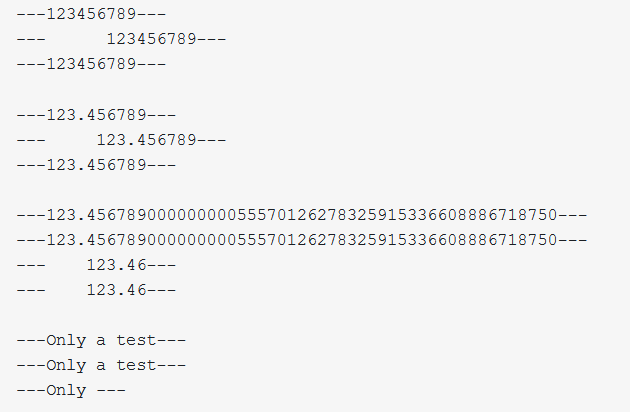
\includegraphics[width=0.8\textwidth]{content/3/chapter5/images/30.png}\\
\end{center}

\hspace*{\fill} \\ %插入空行
\noindent
\textbf{5.6.1.2.4\hspace{0.2cm}类型}

通常,编译器会推断所使用值的类型,但有时需要指定类型。以下是最重要的类型规范:

\begin{itemize}
\item 
字符串: s

\item 
整型:
\begin{itemize}
\item 
b: 二进制格式

\item 
B: 与b相同,但前缀是0B

\item 
d: 十进制格式

\item 
o: 八进制格式

\item 
x: 十六进制格式

\item 
X: 与x相同,但前缀是0X
\end{itemize}

\item 
char和wchar\_t:
\begin{itemize}
\item 
b, B, d, o, x, X: 和整型一样
\end{itemize}

\item 
bool:
\begin{itemize}
\item 
s: true或false

\item 
b, B, d, o, x, X: 和整型一样
\end{itemize}

\item 
浮点:
\begin{itemize}
\item 
e: 指数格式

\item 
E: 和e一样,但是指数用E

\item 
f, F: 定点格式,精度为6

\item 
g, G: 精度6,指数用E
\end{itemize}
\end{itemize}

若不指定类型,则显示如下所示。字符串显示为字符串,十进制格式的整数,字符显示为字符,浮点值显示为\href{https://en.cppreference.com/w/cpp/utility/to_chars}{std::to\_chars}。

有了类型说明符,就可以在不同的数字系统中轻松显示int了。

\begin{lstlisting}[style=styleCXX]
// formatType.cpp

#include <fmt/core.h>
#include <iostream>

int main() {

	int num{2020};
	
	std::cout << "default: " << fmt::format("{:}", num) << '\n';
	std::cout << "decimal: " << fmt::format("{:d}", num) << '\n';
	std::cout << "binary: " << fmt::format("{:b}", num) << '\n';
	std::cout << "octal: " << fmt::format("{:o}", num) << '\n';
	std::cout << "hexadecimal: " << fmt::format("{:x}", num) << '\n';

}
\end{lstlisting}

\begin{tcblisting}{commandshell={}}
default:     2020
decimal:     2020
binary:      11111100100
octal:       3744
hexadecimal: 7e4
\end{tcblisting}

目前为止,我已经格式化了基本类型和字符串。此外,还可以格式化自定义的类型。

\subsubsubsection{5.6.2\hspace{0.2cm}自定义的类型}

要格式化自定义类型,必须为自定义类型特化类\href{https://en.cppreference.com/w/cpp/utility/format/formatter}{std::formatter}。所以,必须实现成员函数的parse和format。

\begin{itemize}
\item 
parse:
\begin{itemize}
\item 
接受parse上下文

\item 
解析parse上下文

\item 
返回格式规范末尾的迭代器

\item 
若发生错误,抛出std::format\_error
\end{itemize}

\item 
format:
\begin{itemize}
\item 
获取应该格式化的值t和格式上下文fc

\item 
根据格式上下文进行格式化

\item 
将输出写入到fc.out()

\item 
返回一个表示输出结束的迭代器
\end{itemize}
\end{itemize}

来把理论应用到实践中吧,先来格式化std::vector。

\hspace*{\fill} \\ %插入空行
\noindent
\textbf{5.6.2.1\hspace{0.2cm}格式化std::vector}

对std::formatter类的第一个特化非常简单,为容器的每个元素指定了格式规范。

\begin{lstlisting}[style=styleCXX]
// formatVector.cpp

#include <iostream>
#include <fmt/format.h>
#include <string>
#include <vector>

template <typename T>
struct fmt::formatter<std::vector<T>> {

	std::string formatString;
	
	auto constexpr parse(format_parse_context& ctx) {
		formatString = "{:";
		std::string parseContext(std::begin(ctx), std::end(ctx));
		formatString += parseContext;
		return std::end(ctx) - 1;
	}
	
	template <typename FormatContext>
	auto format(const std::vector<T>& v, FormatContext& ctx) {
		auto out= ctx.out();
		fmt::format_to(out, "[");
		if (v.size() > 0) fmt::format_to(out, formatString, v[0]);
		for (int i= 1; i < v.size(); ++i) fmt::format_to(out, ", " + formatString, v[i]);
		fmt::format_to(out, "]");
		return fmt::format_to(out, "\n" );
	}

};


int main() {

	std::vector<int> myInts{1, 2, 3, 4, 5, 6, 7, 8, 9, 10};
	std::cout << fmt::format("{:}", myInts);
	std::cout << fmt::format("{:+}", myInts);
	std::cout << fmt::format("{:03d}", myInts);
	std::cout << fmt::format("{:b}", myInts);
	
	std::cout << '\n';
	
	std::vector<std::string> myStrings{"Only", "for", "testing", "purpose"};
	std::cout << fmt::format("{:}", myStrings);
	std::cout << fmt::format("{:.3}", myStrings);

}
\end{lstlisting}

std::vector(第8行)的特化有成员函数parse(第13行)和format(第20行)。parse实际上创建了formatString,应用于std::vector的每个元素(第24和25行),解析上下文ctx(第13行)包含冒号(:)和右大括号(\})之间的字符。最后,函数返回一个指向右大括号(\})的迭代器。成员函数format的工作方式更有趣,格式上下文会返回输出迭代器。有了输出迭代器和函数\href{https://en.cppreference.com/w/cpp/utility/format/format_to}{std::format\_to}, std::vector的元素就能很好地显示出来了。

vector(第35行)的元素有几种格式化方式。第36行显示数字,第37行在每个数字之前写一个符号,第38行将其以3个字符的长度对齐,并使用0填充。第39行以二进制格式显示。剩下的两行输出std::vector的每个字符串。最后,第45行将每个字符串截断为三个字符。

\begin{center}
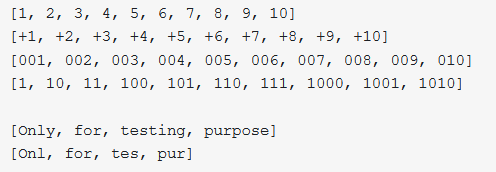
\includegraphics[width=0.8\textwidth]{content/3/chapter5/images/1-8.png}\\
\end{center}

当std::vector元素越来越多的时候,我想添加一个换行符。对于这个用例,我扩展了格式规范的语法。

\begin{lstlisting}[style=styleCXX]
// formatVectorLinebreak.cpp

#include <algorithm>
#include <iostream>
#include <limits>
#include <numeric>
#include <fmt/format.h>
#include <string>
#include <vector>

template <typename T>
struct fmt::formatter<std::vector<T>> {

	std::string systemFormatString;
	std::string userFormatString;
	int lineBreak{std::numeric_limits<int>::max()};
	
	auto constexpr parse(format_parse_context& ctx) {
		std::string startFormatString = "{:";
		std::string parseContext(std::begin(ctx), std::end(ctx));
		auto posCurly = parseContext.find_last_of("}");
		auto posTab = parseContext.find_last_of("|");
		if (posTab == std::string::npos) {
			systemFormatString = startFormatString + parseContext.substr(0, posCurly + 1);
		}
		else {
			systemFormatString = startFormatString + parseContext.substr(0, posTab) + "}";
			userFormatString = parseContext.substr(posTab + 1, posCurly - posTab - 1);
			lineBreak = std::stoi(userFormatString);
		}
		return std::begin(ctx) + posCurly;
	}

template <typename FormatContext>
auto format(const std::vector<T>& v, FormatContext& ctx) {
	auto out = ctx.out();
	auto vectorSize = v.size();
	if (vectorSize == 0) return fmt::format_to(out, "\n");
	for (int i = 1; i < vectorSize + 1; ++i) {
		fmt::format_to(out, systemFormatString, v[i-1]);
		if ( (i % lineBreak) == 0 ) fmt::format_to(out, "\n");
	}
		return fmt::format_to(out, "\n" );
	}

};

int main() {

	std::vector<int> myInts(100);
	std::iota(myInts.begin(), myInts.end(), 1);
	
	std::cout << fmt::format("{:|20}", myInts);
	std::cout << '\n';
	std::cout << fmt::format("{: |20}", myInts);
	std::cout << '\n';
	std::cout << fmt::format("{:4d|20}", myInts);
	std::cout << '\n';
	std::cout << fmt::format("{:10b|8}", myInts);

}
\end{lstlisting}

下面是其工作原理。我支持一个可选的|符号,后面跟着一个数字的格式规范。这个数字表示是否应该引入换行符。我搜索可选的|符号和右大括号\}。出于对程序鲁棒性的考虑,第21和22行查找最后一个符号。有了|和\}的索引,就可以创建字符串systemFormatString和useFormatString(第24至29行)。成员函数格式使用systemFormatString,并将其应用于vector的每个元素。当满足(i \% lineBreak == 0)条件(第41行)时,就进行换行。

第53行显示一行中有20个元素,并使用换行符,当然可以做得更好。格式规范为\{:|20\}(第55行)在每个数字前加一个空格。另外,第57行将每个元素对齐为四个字符。最后一行每行显示8个数字,将元素以8个字符对齐,并显示:\{:10b|8\}。

屏幕截图显示了std::vector的可读格式化元素。

\begin{center}
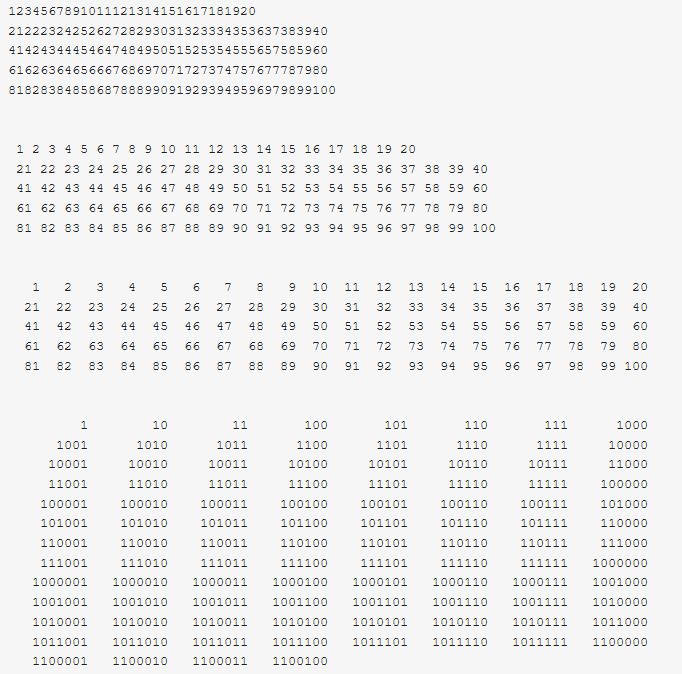
\includegraphics[width=1.0\textwidth]{content/3/chapter5/images/31.png}\\
\end{center}

\begin{tcolorbox}[breakable,enhanced jigsaw,colback=mygreen!5!white,colframe=mygreen!75!black,title={总结}]
	
\begin{itemize}
\item 
格式化库提供了替换printf类函数的安全且可扩展的方案,并扩展了I/O流。

\item 
格式规范允许定填充字母和文本对齐、设置符号、指定数字的宽度和精度,以及指定数据类型。

\item 
有了parse和format函数,就可以根据需要调整自定义类型的格式。
\end{itemize}
	
\end{tcolorbox}

\newpage




